\section{Background} \label{sec:background}

\vspace*{-0.2cm}

This section describes the main concepts related to the design and implementation of Semantic Restful APIs and the process of selecting an API functionality.

\paragraph{Semantic RESTful services}
Combining REST with Semantic Web and Linked Data is a promising path since it enables the description of APIs that can change without breaking client applications. These APIs advertise their available state transitions, therefore enabling automatic composition to create high level services~\cite{alarcon2015rest}. Smart software agents can then automatically discover the suite of operations to realize complex workflows and even make APIs compatible with voice assistants. This is achieved by semantically enriching the data and operations of REST systems with Semantic Web ontology technologies and by linking resources to other resources.

\subsection{Selecting an API functionality level}\label{sec:maturityLevel}

Today, Web systems offer a wide range of functionalities. For example, they may offer multiple media types or a single one, comply with the HTTP protocol or use it as a transfer protocol, or even semantically describe their resources. This diversity can make the process of comparing and selecting the minimum set of features to be implemented in a company very time-consuming. Maturity models have been proposed as a solution to this problem~\cite{paulk1993capability}~\cite{7195633}.

In companies, architects use them to decide features which must be supported by their APIs. In general, a maturity model is a scale that represents the compliance of a technology with a given architecture. To reach a level, a technology must meet each constraint of the targeted level and the previous levels.
Currently, the de-facto standard in industry is the Richardson Maturity Model \cite{RichardsonMaturityModel}, which targets building REST APIs. However, we recommend using the WS3 maturity model \cite{7195633} as it combines the models proposed by Richardson, and SoHA \cite{SoHA}, and extend them with semantic and documentation constraints.

\vspace*{-0.5cm}

\subsubsection{The WS3 maturity model}

In \cite{7195633}, authors describe the WS3 maturity model for classifying Semantic REST Web APIs. 
It classifies APIs along three independent dimensions: \textit{design}, \textit{profile} and \textit{semantic}, as shown in Fig. \ref{WS3}.

\begin{wrapfigure}{l}{0.52\textwidth}
\vspace{-0.9cm}
\caption{ WS3 Maturity Model (from \cite{7195633})}
  \begin{center}
    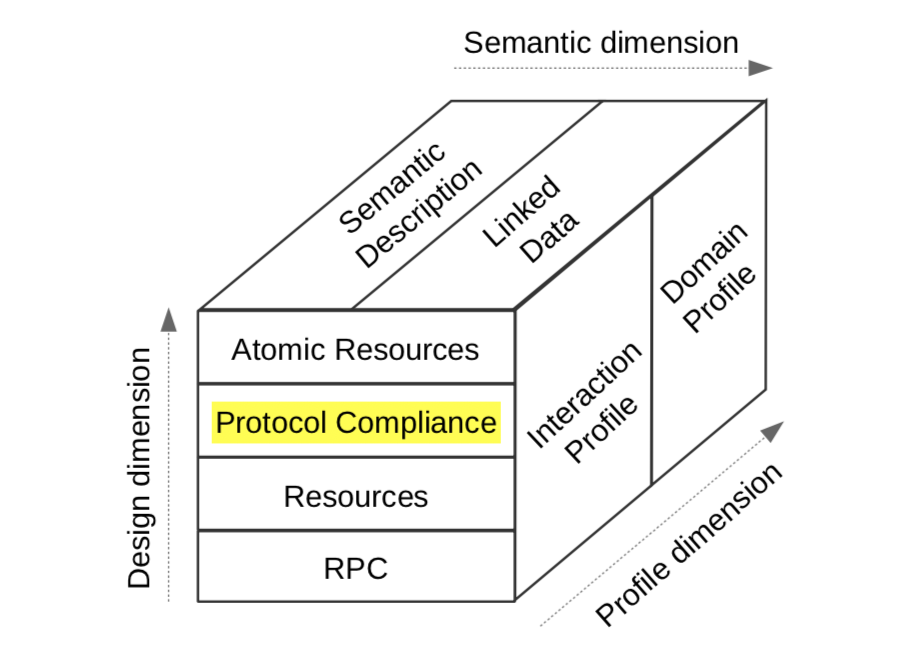
\includegraphics[width=0.4\textwidth]{figures/ws3-maturity-model.png}
  \end{center}
  \label{WS3}
  \vspace{-0.9cm}
\end{wrapfigure}

%\vspace*{-0.5cm}
%\begin{figure}[ht]
%  \caption{\vspace*{-0.5cm} WS3 Maturity Model (from \cite{7195633})}
%  \centering
%  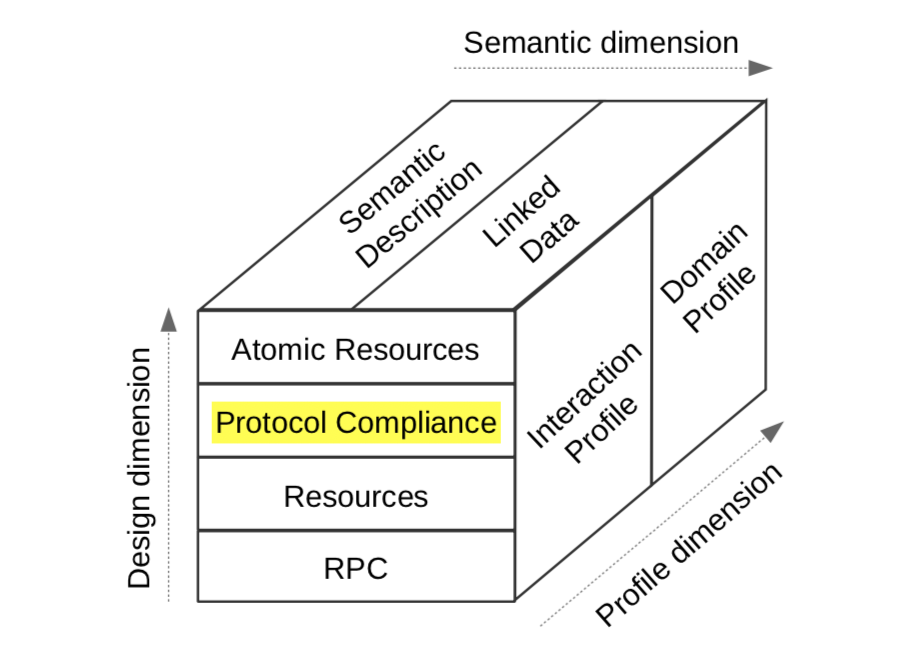
\includegraphics[width=0.47\textwidth]{figures/ws3-maturity-model.png}
%  \label{WS3}
%\end{figure}
%\vspace*{-0.5cm}
The \textbf{design dimension} represents the different modeling strategies adopted for designing the technical access to a Web API through four levels:
(i) RPC-like, (ii) resources have dedicated URI and the API is stateless, (iii) operations on a resource are mapped to HTTP verbs in compliance with the protocol and (iv) the smallest data unit that can be handled by operations is the resource.

The \textbf{profile dimension} reflects the quality of documentation that can be interpreted by software agents through two levels. The first level: \textit{interaction profile}, requires the description of all available HTTP operations and how to trigger them. The second level: the \textit{domain profile}, requires the description of domain specific details such as the order of operation execution, pre- and post-conditions, business constraints, etc.

The \textbf{semantic dimension} represents the use of semantic technologies through two levels. To reach the \textit{Semantic Description level}, an API must semantically describe properties and operations of resources. The next level: \textit{Linked Data}, is reached when the API semantically describes relationships between resources.

\paragraph{Usage}
In their paper \cite{7195633}, Salvadori \emph{et al.} propose to rate systems along each dimension independently, with a score going from 0 to the number of levels in the dimension.
For example, a non-documented API with no semantic support that reach level 3 of the Richardson Maturity Model will be rated D3-S0-P0\footnote{D3-S0-P0: Atomic Resources Design, no Semantic Description, no Profile description}. As another example, a system that supports HATEOAS and provides a swagger-like documentation along with the data is rated D3-S0-P2\footnote{D3-S0-P2: Atomic Resources Design, no Semantic Description, Domain Profile}.
\vspace*{-0.5cm}
\subsection{Discussion on the WS3 maturity level}
\vspace*{-0.2cm}

From our experience at FABERNOVEL, we noticed two limitations to the applicability of the maturity model to a wider audience. These limitations are related to the \textit{Atomic Resources level} and the granularity of the WS3 level.

According to WS3, the \textit{Atomic Resources} constraint requires that the smallest data unit handled by operations is the resource.
Respecting this constraint may introduce negative properties on the API.
Let us consider an API handling insurance contracts which offers read and update operations on the postal address, email address and insurance manager. 
Two solutions can be considered to respect the \textit{Atomic Resources} constraint. 
The first solution is to create one resource, where every properties can be modified at once, which increases the risk of concurrent modification. 
With this solution, the API would have two operations. 
The second solution is to create one resource for each concept: contract, email address, postal address and the manager. The API would have eight operations. This solution increases dramatically the number of operations which complexify the documentation and maintainability.
Another solution would be to create one resource with four operations: (i) read, (ii) update email, (iii) update postal address and (iv) update manager. 
This solution lowers the concurrency risk while maintaining a reasonable complexity and offering meaningful operation names. Unfortunately this solution breaks the \textit{Atomic Resources constraint}. We therefore argue that respecting this last constraint may not always lead to better API quality.

The second limitation relates to the granularity of the maturity levels. Indeed, each level implies more than one feature. This granularity allows for a coarse-grained categorization of systems. 
However, to precisely differentiate systems based on the features they implement, a deeper study is needed. 
Given two systems that reach P1, which means they describe all available HTTP operations and how to trigger them, one might also describe its authentication process and errors whereas the second does not. 
And yet they reach the same maturity level. 
We therefore argue for a finer grain categorization of API.